\documentclass{article_saj}
\pagestyle{myheadings}
\usepackage{graphicx,saj,multicol,subeqnarray}
\usepackage{natbib}
\usepackage{float}
\usepackage{xcolor}
\usepackage{widetext}
\usepackage{url}
\usepackage{bm}
\usepackage{amsfonts,amssymb,amsmath}
\usepackage[T1]{fontenc}
\usepackage[utf8]{inputenc}
\usepackage{microtype}
\definecolor{xlinkcolor}{cmyk}{1,0.6,0,0}
\usepackage[bookmarks=false,pdfnewwindow=true,colorlinks=true,linkcolor=xlinkcolor,citecolor=xlinkcolor,filecolor=xlinkcolor,urlcolor=xlinkcolor,final=true]{hyperref}
\def\papertype{\ \hfill\ Original Scientific Paper}
\def\udc{52}
\setcounter{publno}{000}
\setcounter{publyear}{2026}
\setcounter{page}{1}
\setcounter{firstpage}{1}
\setcounter{lastpage}{10}
\citestyle{kluwer}
\setcounter{footnote}{0}
\renewcommand{\thefootnote}{\fnsymbol{footnote}}
\begin{document}
\parindent=.5cm
\baselineskip=3.8truemm
\columnsep=.5truecm
\newenvironment{lefteqnarray}{\arraycolsep=0pt\begin{eqnarray}}{\end{eqnarray}\protect\aftergroup\ignorespaces}
\newenvironment{lefteqnarray*}{\arraycolsep=0pt\begin{eqnarray*}}{\end{eqnarray*}\protect\aftergroup\ignorespaces}
\newenvironment{leftsubeqnarray}{\arraycolsep=0pt\begin{subeqnarray}}{\end{subeqnarray}\protect\aftergroup\ignorespaces}
\markboth{\eightrm NETWORK-TRIGGERED CULTURAL IGNITION}{\eightrm M. SHATOKHIN}
\begin{strip}
{\ }
\vskip-1cm
\publ
\type
{\ }
\title{NETWORK-TRIGGERED CULTURAL IGNITION AS A CANDIDATE GREAT FILTER}
\authors{M. Shatokhin$^{1}$}
\vskip3mm
\address{$^1$National University ``Kyiv Aviation Institute'', Kyiv, Ukraine\\ ORCID: 0000-0003-0028-6208}
\Email{n.shatokhin@gmail.com}
\summary{The abundance of potentially habitable planets does not directly determine the abundance of technological societies: a biosphere must also cross a transition from individual intelligence and local traditions to persistent, open-ended cumulative culture. We integrate a continuous-feedback agent-based metapopulation model with archaeological and conditional Galactic analyses. Complementary skills are distributed across groups, and technological ignition depends on inter-group information flow, multi-model recombination, teaching and cultural selection on cognition. A dense phase experiment (100 replicates per point) produces a duration-dependent transition, with estimated 50\% ignition thresholds of 0.095, 0.061 and 0.040 for the probability of sampling an external cultural model during contact phases lasting 1000, 1500 and 2000 years. In a separate, coarser ablation grid, removal of recombination, teaching or infrastructure feedback produced no persistent ignitions within the tested domain; removal of cultural selection on cognition shifted the transition beyond the scanned range. An archaeological compatibility analysis identifies a procedural-complexity change point at 525 ka; the temporal association persists under date sampling, source- and site-cluster bootstrap, leave-one-cluster-out tests, baseline changes and 10,000 temporal permutations, but does not identify network connectivity as the cause. Nine network architectures shift the median ignition threshold from 0.056 for global mixing to 0.143 for modular bridge networks. Finally, a Poisson embedding converts the local transition into conditional constraints on successful pre-human ignition events. This does not establish that humanity is first or estimate extraterrestrial abundance; it quantifies the joint rarity of complex life, cultural opportunities and persistent ignition required for this mechanism to act as a candidate Great Filter.}
\keywords{Extraterrestrial intelligence -- Astrobiology -- Methods: numerical -- Methods: statistical -- Galaxy: evolution}
\end{strip}
\tenrm
\indent\footnotetext[0]{\copyright\ 2026 The Author. Published by Astronomical Observatory of Belgrade and Faculty of Mathematics, University of Belgrade. This open access article is distributed under CC BY-NC-ND 4.0 International licence.}
\renewcommand{\thefootnote}{\arabic{footnote}}

\section{INTRODUCTION}

Cosmic planet-formation histories imply that many rocky planets may pre-date the Solar System, while exoplanet surveys permit a large population of rocky habitable-zone candidates \citep{behroozi2015,bryson2021}. The resulting astrobiological question is not only whether life and intelligence evolve, but whether intelligence reliably becomes a technological society capable of generating detectable technosignatures. Recent reassessments of evolutionary hard-step reasoning likewise emphasize environmental windows and unresolved late transitions \citep{mills2025}. This distinction is central to the Great Filter and Fermi-paradox literature, in which the relevant uncertainty is the product of several poorly known biological and social transitions rather than planet abundance alone \citep{kipping2020,schleicher2023,shkurko2024}.

Cumulative cultural evolution permits information to persist, improve and recombine beyond the inventive capacity of any single individual \citep{mesoudi2018}, while structured populations can promote combinatorial cultural systems \citep{kirby2022}. Social learning and tool traditions are not uniquely human: chimpanzees can acquire socially transmitted solutions they fail to innovate alone, and cultural repertoire complexity covaries with population connectivity \citep{vanleeuwen2024,gunasekaram2024}. The unresolved transition is therefore not from non-intelligence to intelligence in a single step, but from local traditions to a self-maintaining network that combines distributed knowledge.

Previous cultural-evolution models show that network architecture, fragmentation, population size, teaching and recombination can affect accumulation \citep{derex2015,derex2018,cantor2021}. Recent astrobiological work has independently proposed symbolic language as an algorithmic bottleneck in a nested Great Filter \citep{prokopenko2026}. The distinctive contribution here is the integration of a mechanistic stochastic metapopulation model, systematic ablations and topology experiments, an archaeological compatibility test and a conditional cosmic population model in one reproducible framework. We ask two linked questions: under what local network conditions does a technological regime become persistent, and how rare must successful cultural ignition be for humanity to plausibly belong to the first Galactic wave? Fig. \ref{fig:1} summarises the local-to-cosmic logic of the analysis.

\begin{figure*}[t]
\centering
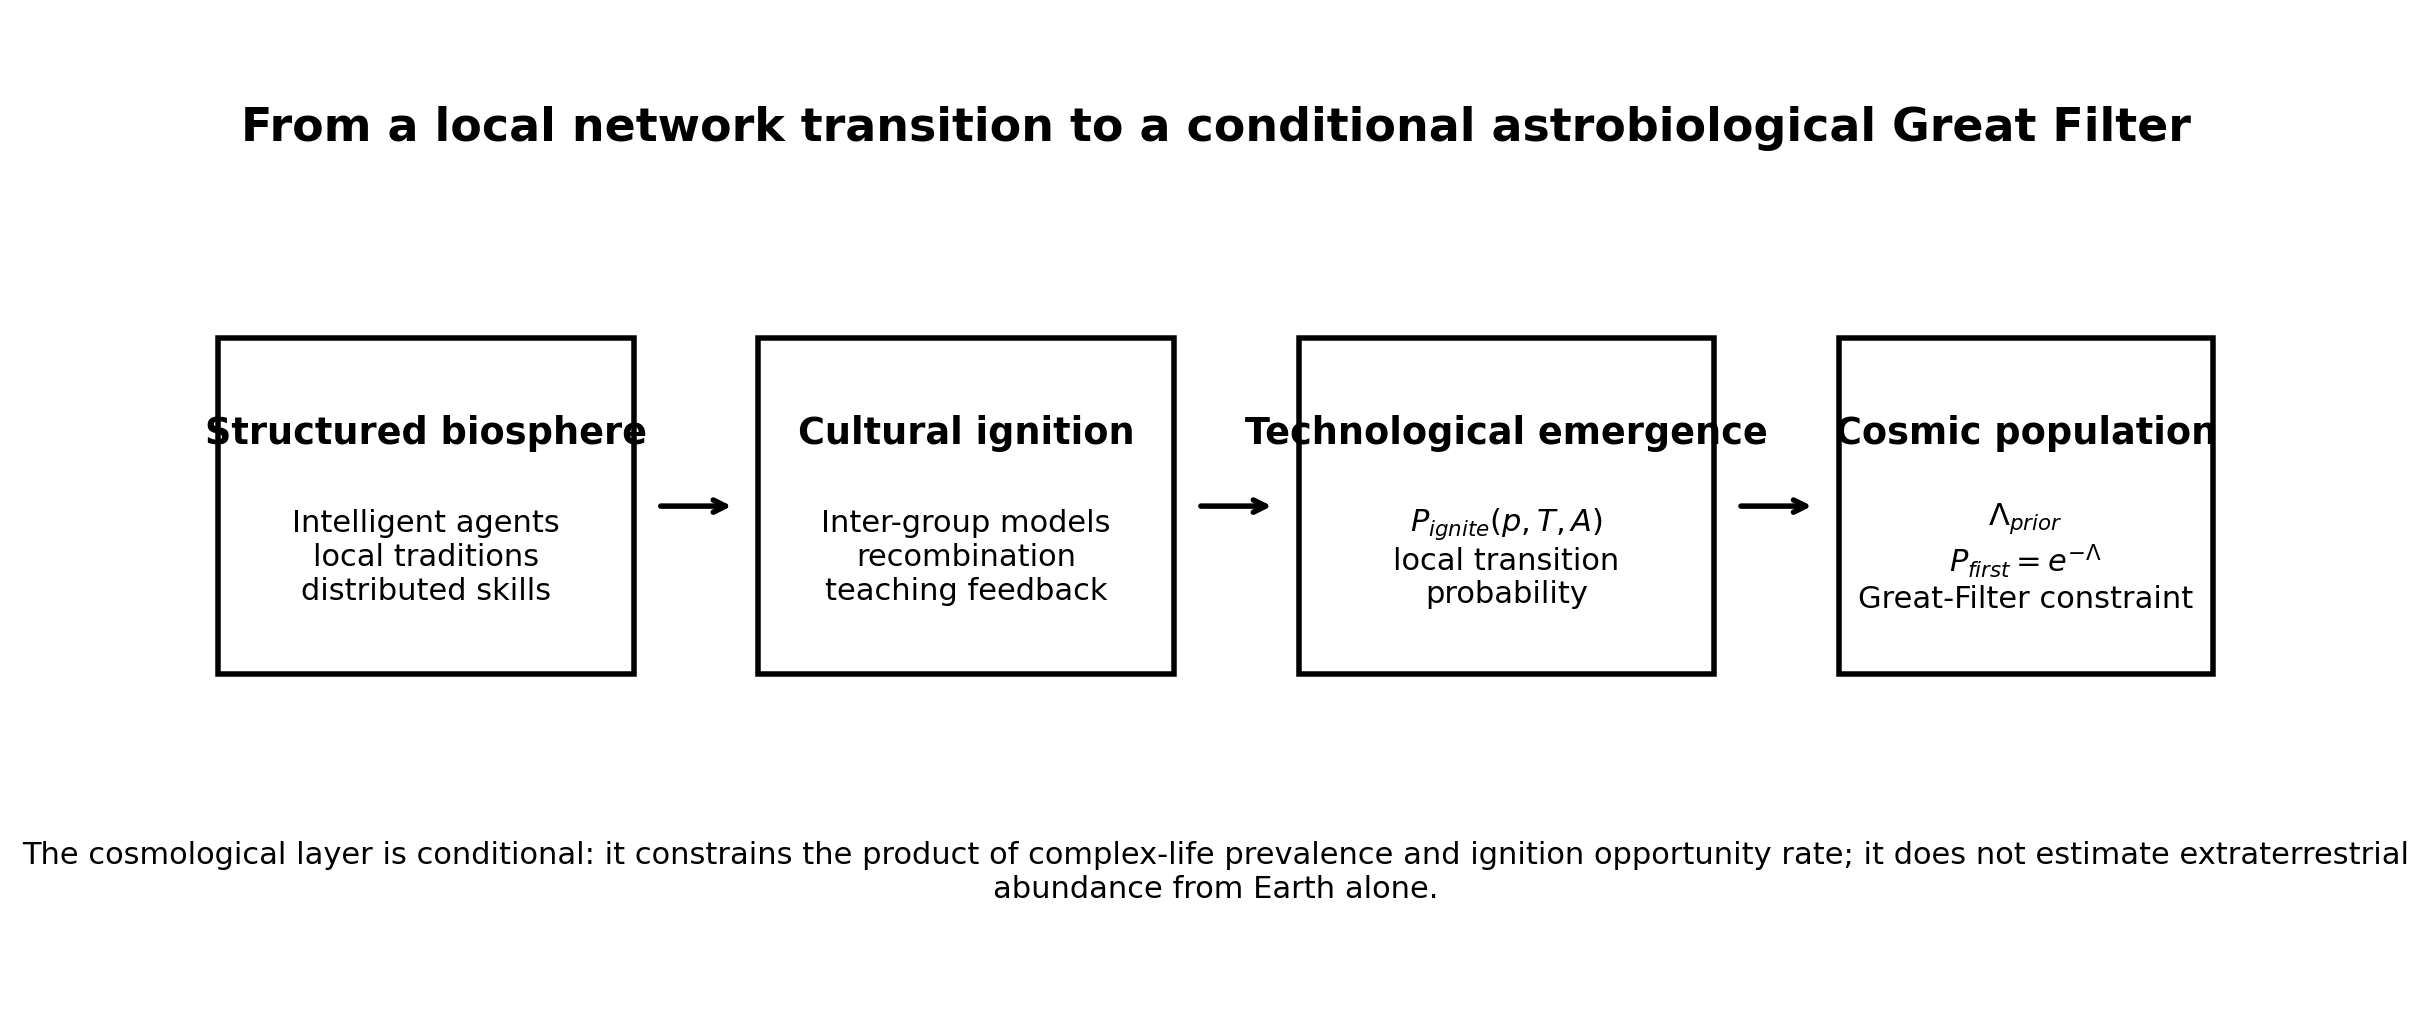
\includegraphics[width=0.94\textwidth]{figures/fig1.png}
\caption{Conceptual linkage from distributed cultural knowledge to a conditional Great-Filter constraint.}
\label{fig:1}
\end{figure*}

\section{MODEL AND METHODS}

\subsection{Structured population and cultural transmission}

The reference metapopulation contains 16 groups of 20 agents. Each agent carries a continuous cognitive trait and six cultural domains with five prerequisite levels per domain. Groups preferentially innovate in different ecological specialities, creating distributed complementary knowledge. Cognition is inherited with Gaussian mutation. Reproductive weight increases with repertoire and decreases with the energetic cost of cognition:

\begin{equation}
W_i=\exp\!\left(b_S S_i-c_B B_i^2\right).
\label{eq:fitness}
\end{equation}

Each learner samples local and external cultural models. During a contact phase, the probability that any sampled model belongs to another group is \(p_{\rm ext}\). A learner can take the best observed level independently in each domain, which permits recombination across multiple specialists. High levels require successful sequential acquisition of all prerequisites.

Teaching quality, the number of models sampled, innovation productivity and group learning infrastructure are smooth functions of actual repertoire breadth, teacher density and domain diversity. This design is motivated by formal work on high-fidelity social learning and experimental evidence that teaching and language improve transmission of complex tool-making sequences \citep{montrey2020,morgan2015}. No variable equivalent to the technological outcome criterion appears inside these feedbacks; the former programmed institutional switch was removed.

\subsection{Outcome and phase experiments}

The primary individual diagnostic requires a total repertoire of at least 16 levels and developed skills in at least five of six domains. Persistent ignition requires more than half of agents to meet this diagnostic during at least 45 of the final 50 generations, with final-period mean repertoire above 18. Permissive and strict definitions test threshold robustness.

The dense phase experiment varied \(p_{\rm ext}\) from 0.002 to 0.12 and contact duration across 40, 60 and 80 generations (1000, 1500 and 2000 years at 25 years per generation). Each point used 100 independent stochastic seeds. Wilson intervals summarize binomial uncertainty. Binomial generalized linear models with contact, duration and interaction estimate \(p_{50}\), the external-model probability associated with 50\% persistent ignition. Fig. \ref{fig:2} displays the fitted duration-dependent phase curves and Wilson uncertainty bands.

\begin{figure*}[t]
\centering
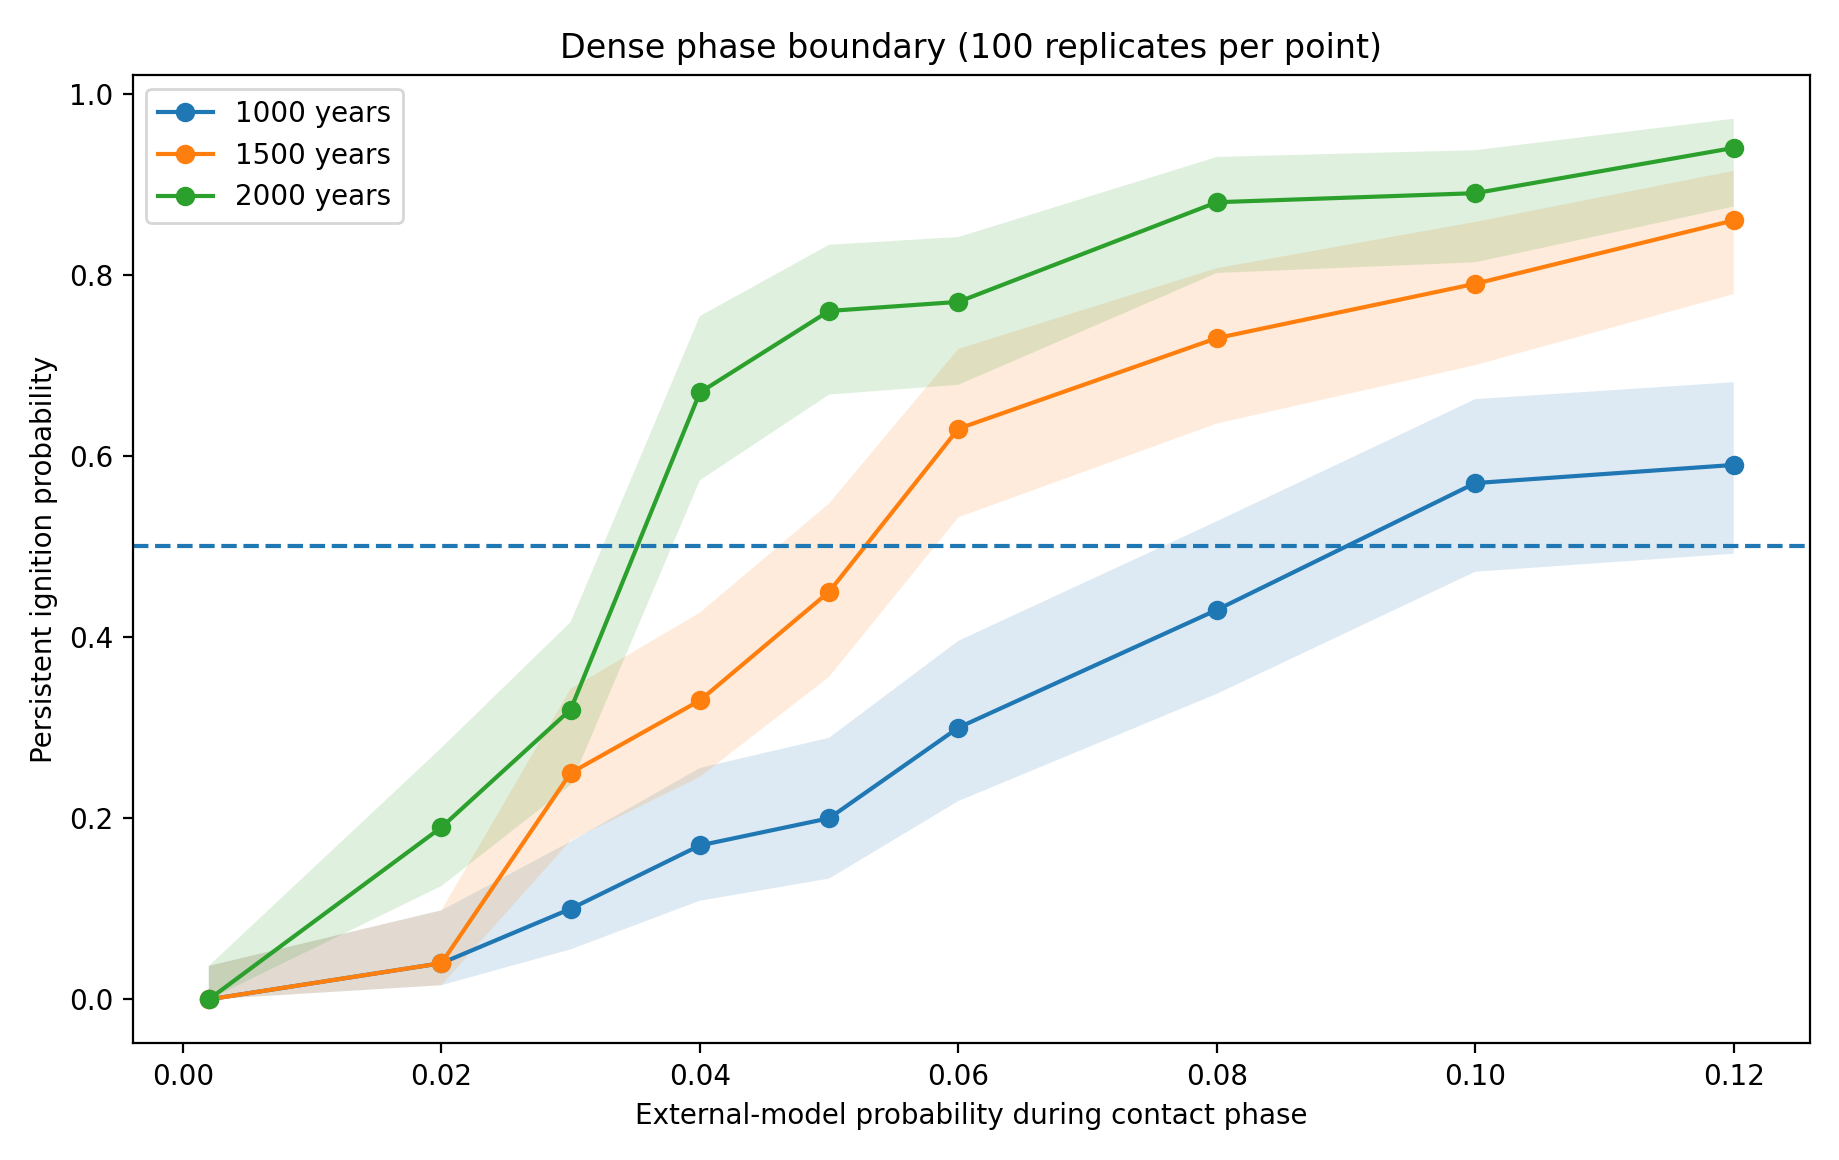
\includegraphics[width=0.94\textwidth]{figures/fig2.png}
\caption{Persistent-ignition probability across contact strength and duration. Shaded bands show Wilson 95\% intervals.}
\label{fig:2}
\end{figure*}

\subsection{Expanded ablations and global sensitivity}

Ablations were evaluated on a grid of \(p_{\rm ext}\) = 0.03, 0.06, 0.10 and 0.16 and durations of 1000, 1500 and 2000 years, with 50 replicates per condition. Components removed separately were multi-model recombination, active teaching, smooth infrastructure feedback and cultural selection on cognition. A no-contact null used 300 replicates. Claims of necessity are explicitly restricted to this tested domain.

Global sensitivity used a 256-point Latin-hypercube design over 14 parameters with three stochastic replicates per point. In-sample random-forest permutation importance and Spearman association provide an exploratory parameter ranking; they are not interpreted as out-of-sample predictive importance or as a formal Sobol variance decomposition. Fig. \ref{fig:3} compares the full model with the expanded ablation grids.

\begin{figure*}[t]
\centering
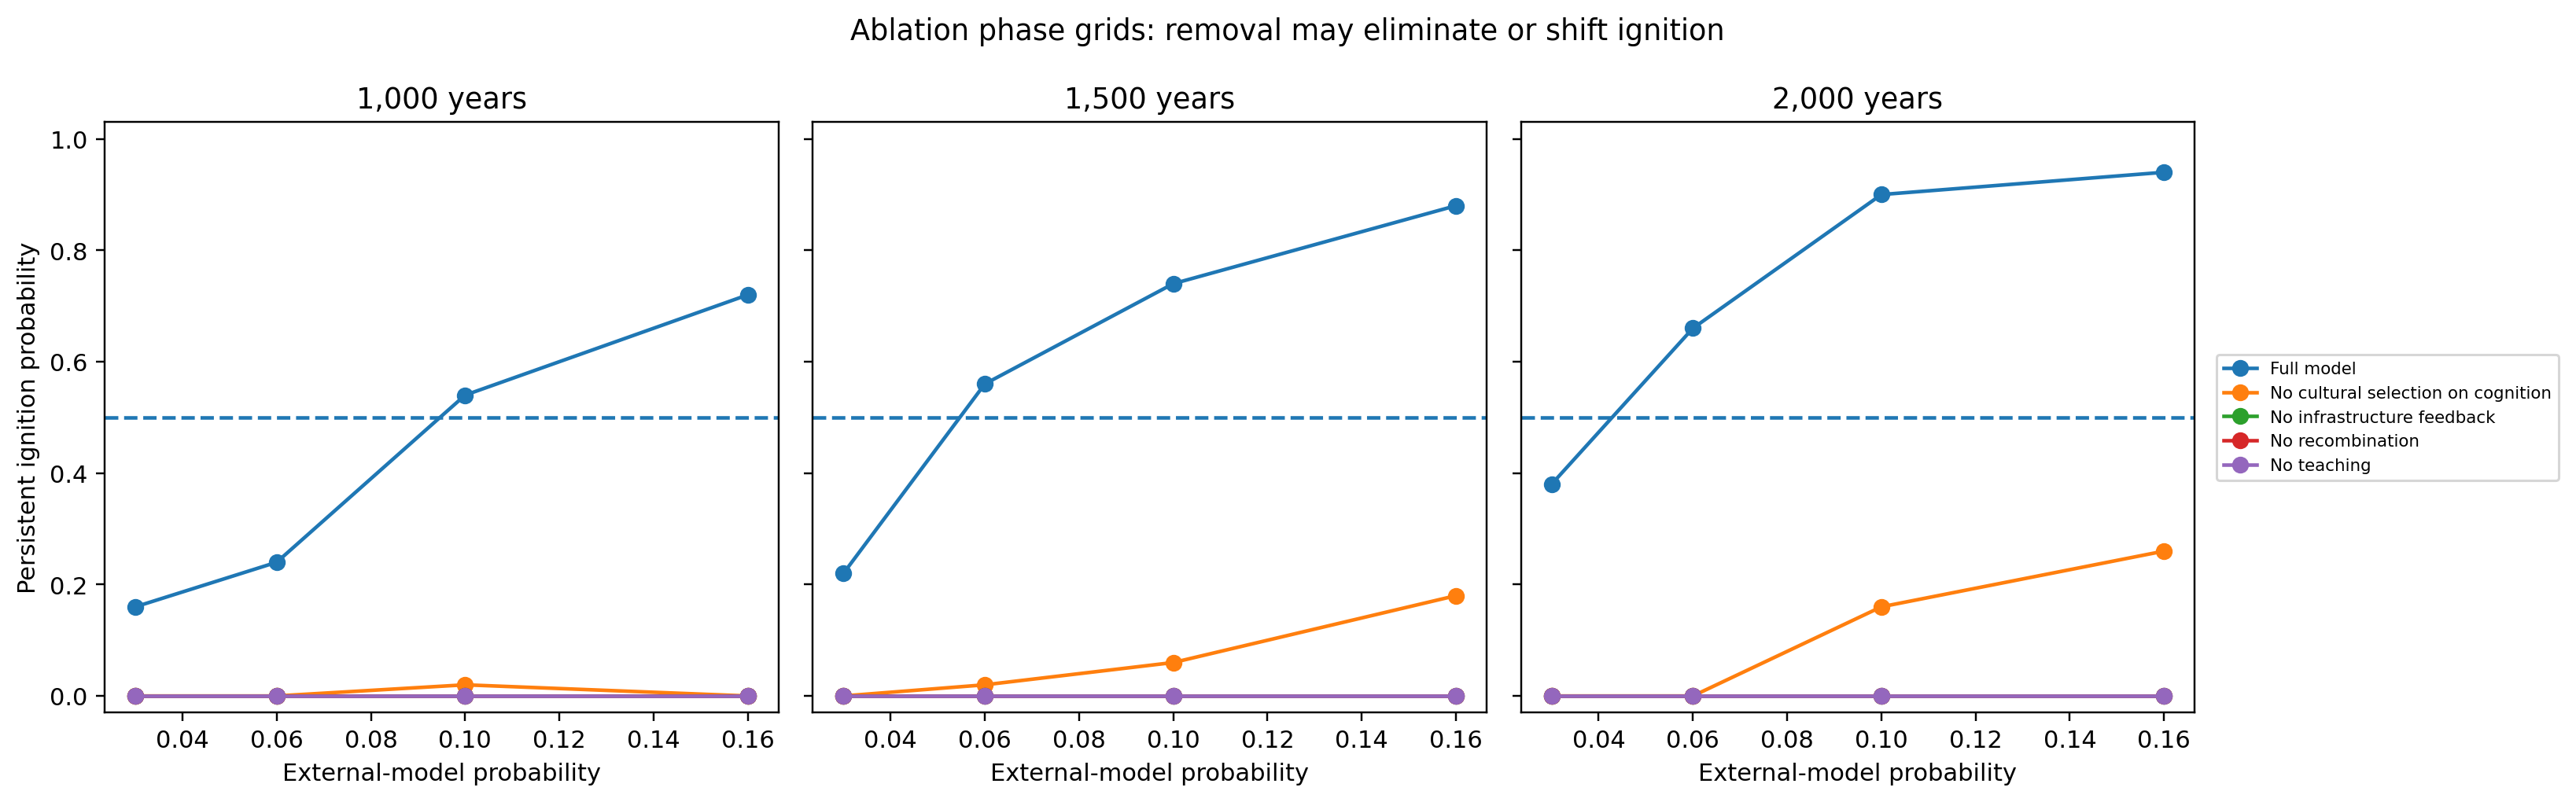
\includegraphics[width=0.94\textwidth]{figures/fig3.png}
\caption{Expanded ablation phase grids. Removal of recombination, teaching or infrastructure feedback eliminated ignition throughout the tested range; cognition selection mainly shifted the transition.}
\label{fig:3}
\end{figure*}

\subsection{Archaeological compatibility and robustness}

We reanalysed the open procedural-unit dataset of \citet{paige2023,paige2024}. The source contains 155 records and 33 binary manufacturing operations. The archived preprocessing script retains rows with \texttt{Arch=1} and \texttt{Single.Chain=yes}, sums the 33 \texttt{PU.*} indicators, and assigns each record the midpoint of its reported age interval. This yields 64 dated archaeological single-chain sequences. Ten non-archaeological primate and experimental records in the source data define a conservative comparison maximum of six procedural units. A two-regime Bernoulli change point was optimised on a 25-ka grid.

Robustness analyses included 10,000 temporal permutations; Monte Carlo sampling within reported age intervals; row, source and site cluster bootstraps; leave-one-source and leave-one-site-out analysis; procedural baselines of five, six and seven units; and fixed temporal boundaries from 500 to 700 ka. This section is termed an archaeological compatibility analysis, not a direct calibration of prehistoric contact. ROAD transport-distance fields provide an appropriate target for future direct calibration but were not used numerically here \citep{kandel2023}. Long-distance raw-material transfer is an established proxy for maintaining social connections \citep{pearce2014}, and the present generative comparison follows the broader theory-to-data workflow advocated by \citet{deffner2024}. Fig. \ref{fig:4} summarises the uncertainty and cluster-robustness analyses.

\begin{figure*}[t]
\centering
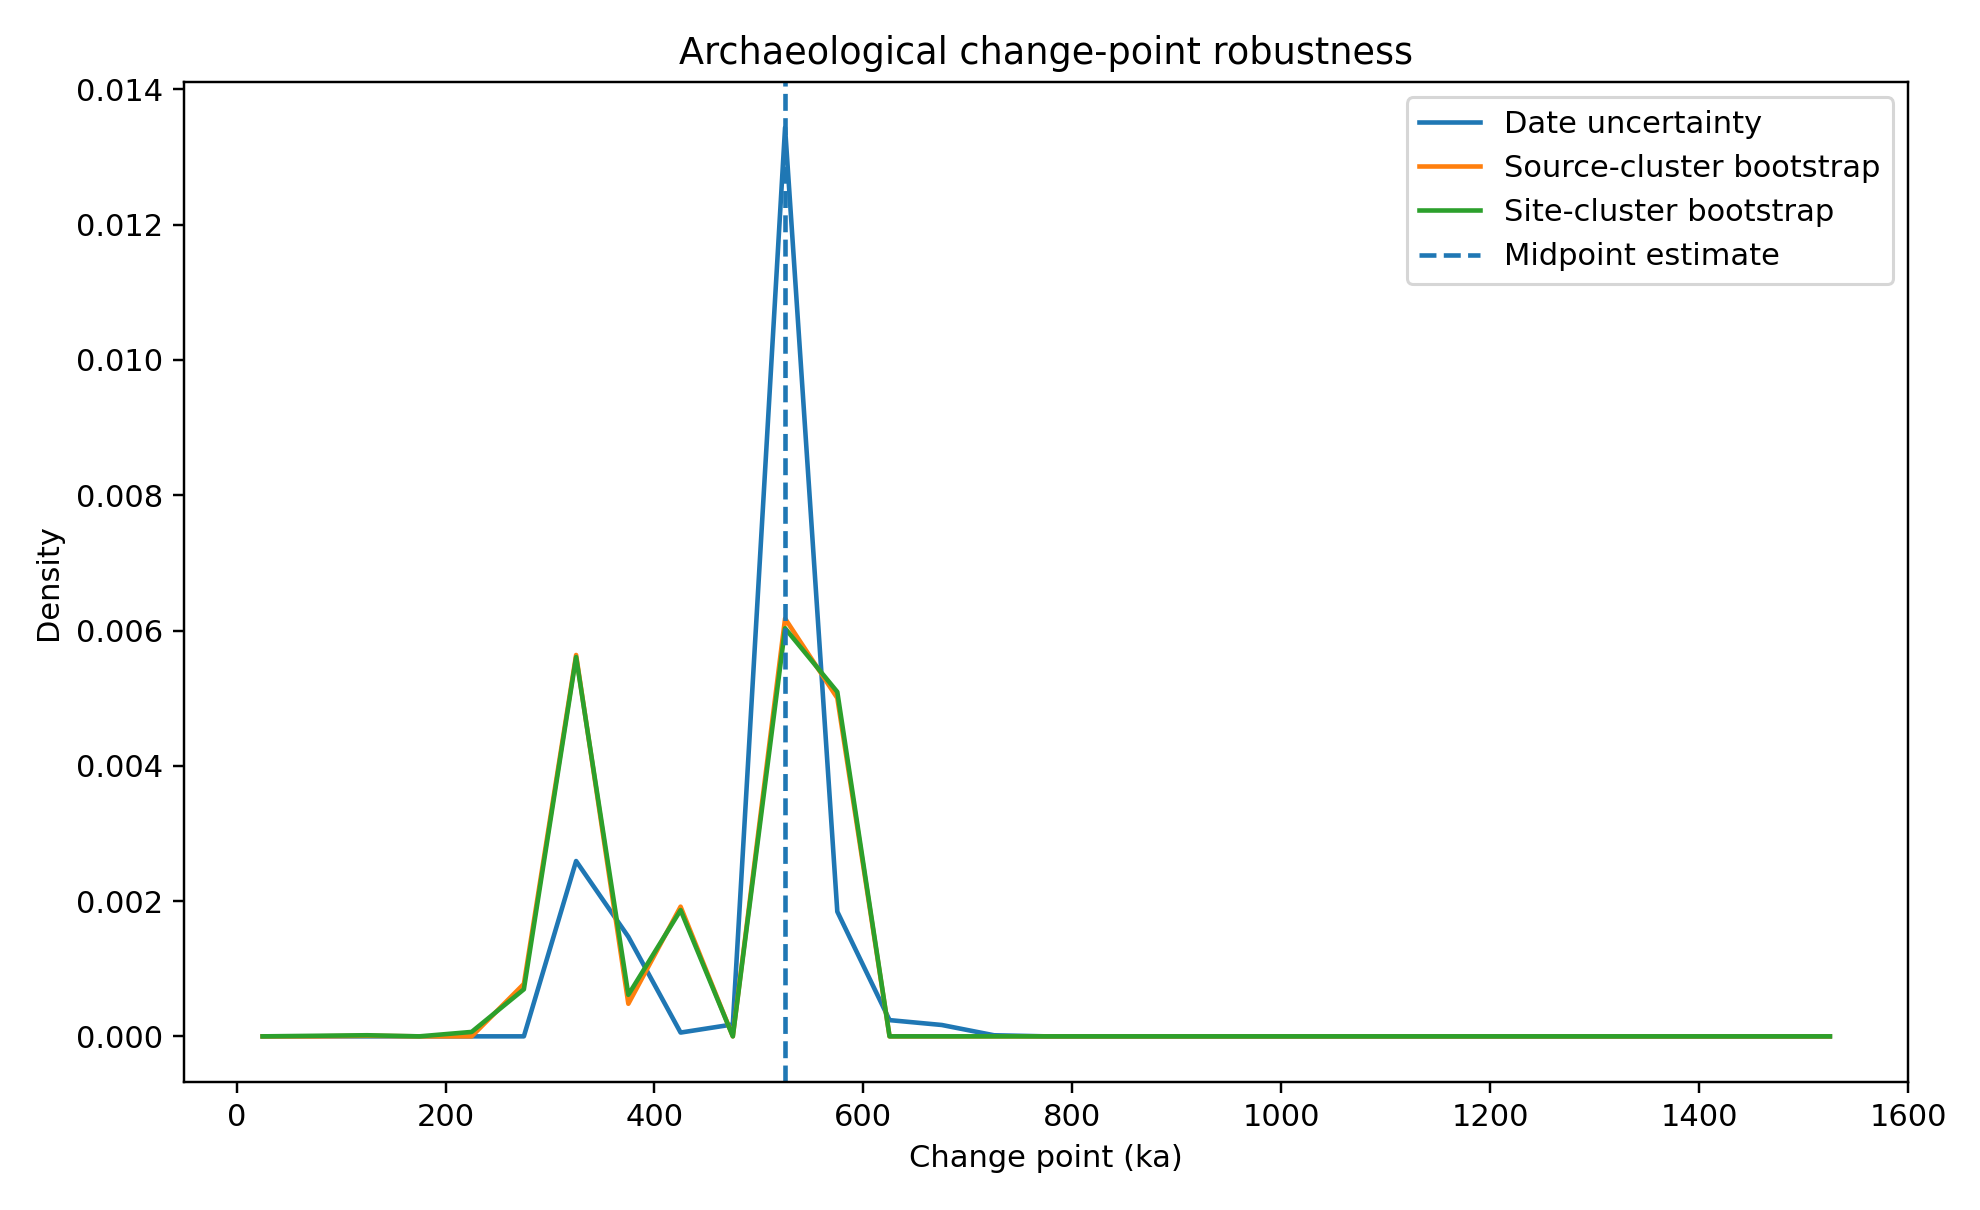
\includegraphics[width=0.94\textwidth]{figures/fig4.png}
\caption{Robustness of the archaeological change point to date uncertainty and source- or site-cluster resampling.}
\label{fig:4}
\end{figure*}

\subsection{Population architecture and network topology}

Population-architecture robustness was tested with fixed total population, fixed local group size and fixed group count. These exploratory ensembles used eight replicates per point and are reported with censoring where the 50\% level lay outside the scanned range. They test whether the transition is specific to 16 groups of 20 agents, not an asymptotic finite-size law.

Nine group-level topologies were evaluated: complete, ring, periodic lattice, Erd\H{o}s--R\'enyi \citep{erdos1959}, Watts-Strogatz small-world \citep{watts1998}, Barab\'asi--Albert scale-free \citep{barabasi1999}, modular stochastic-block \citep{holland1983}, a wheel graph (one hub plus a peripheral cycle) and a distance-weighted gravity network. Graph construction used NetworkX \citep{hagberg2008}. Deterministic topologies used 120 agent seeds per contact. For each stochastic topology and contact level, 20 independently generated graph realisations were each paired with eight agent seeds. Contact-stratified bootstrap resampling therefore propagates graph-realisation uncertainty into \(p_{50}\) intervals. Fig. \ref{fig:5} reports the resulting threshold distributions.

\begin{figure*}[t]
\centering
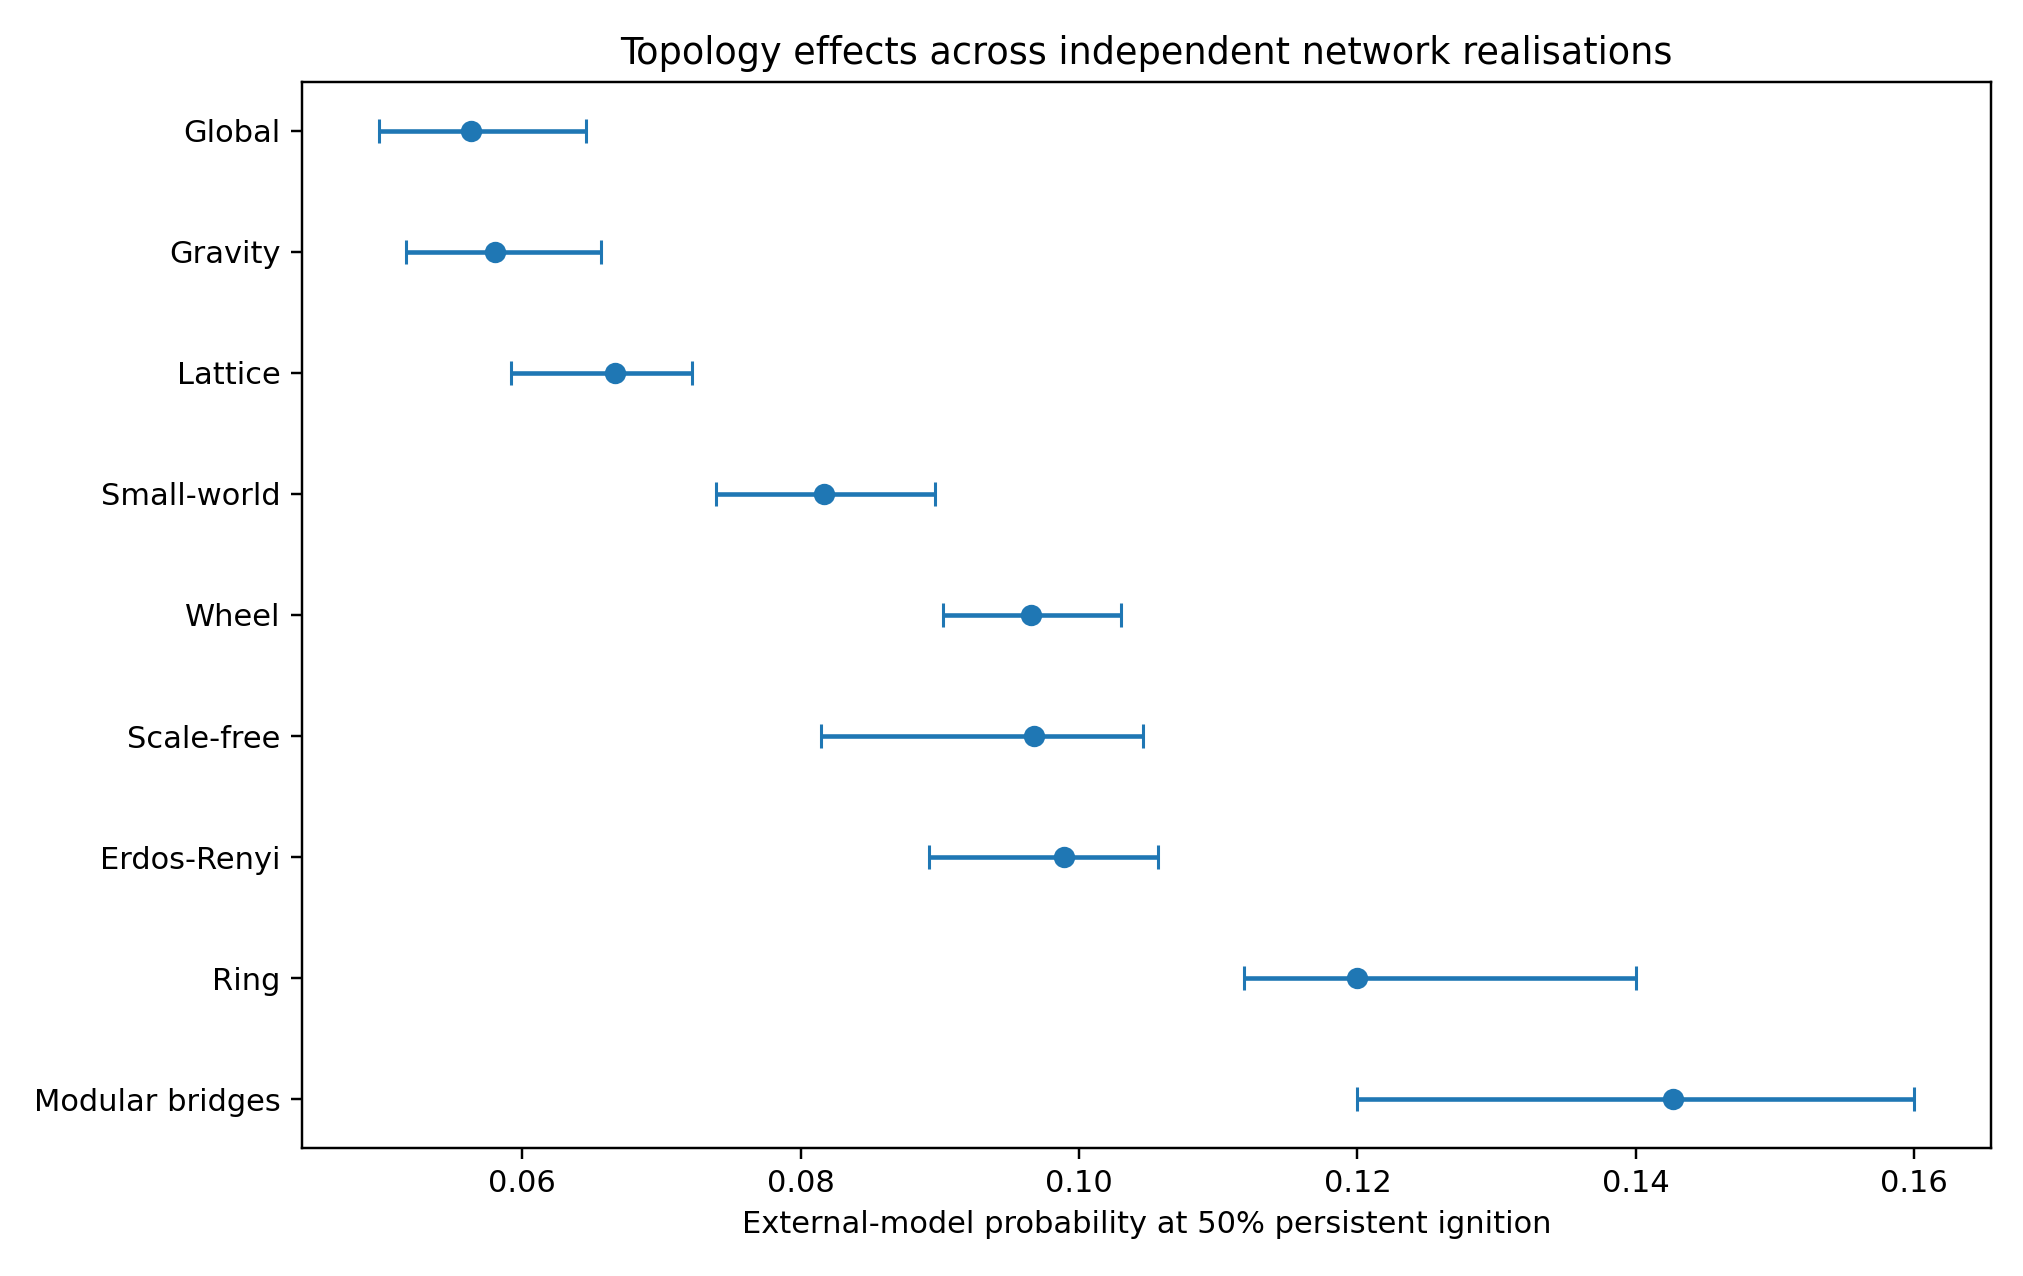
\includegraphics[width=0.94\textwidth]{figures/fig5.png}
\caption{Network-topology thresholds with 95\% bootstrap intervals. Stochastic topologies include independent graph realisations at every contact condition.}
\label{fig:5}
\end{figure*}

\subsection{Conditional cosmic embedding}

The local agent model supplies \(P_{\rm ignite}\)(p,T,A), the probability of persistent cultural ignition for contact strength p, duration T and network architecture A. We do not infer the extraterrestrial distribution of p, T or A from Earth. Instead, we embed \(P_{\rm ignite}\) in a transparent Poisson population model to derive conditional Great-Filter constraints through Eqs. (\ref{eq:prior}) and (\ref{eq:first}).

\begin{equation}
\Lambda_{\rm prior}=N_{\rm HZ} f_{\rm complex}\,\bar{E}\,r_{\rm opp}P_{\rm ignite}.
\label{eq:prior}
\end{equation}

\begin{equation}
P_{\rm no\,prior}=\exp\!\left(-\Lambda_{\rm prior}\right).
\label{eq:first}
\end{equation}

\(N_{\rm HZ}\) is the number of rocky habitable-zone planets under consideration; \(f_{\rm complex}\) is the fraction that reach complex animal-grade biospheres; \(\bar{E}=\mathbb{E}[E\mid\mathrm{complex\ life}]\) is the mean pre-present duration for which such a biosphere is eligible to ignite, conditional on complex life having arisen; and \(r_{\rm opp}\) is the rate of ecological-demographic opportunities per eligible biosphere per Gyr. This conditional definition prevents complex-life rarity from being counted both in \(f_{\rm complex}\) and inside \(\bar{E}\). We do not infer \(\bar{E}\) from the present data. It is an explicit scenario parameter: the reported fiducial calculation uses \(\bar{E}=4\) Gyr, while supplementary sensitivity calculations use 1, 4 and 10 Gyr. \(N_{\rm HZ}\) is scanned from \(10^8\) to \(10^{10}\) to span major occurrence-rate uncertainty \citep{behroozi2015,bryson2021}. Numerical arrays and scientific calculations used NumPy and SciPy \citep{harris2020,virtanen2020}.

\section{RESULTS}

\subsection{A duration-dependent stochastic ignition boundary}

In the dense phase experiment, the estimated primary \(p_{50}\) declined from 0.095 at 1000 years to 0.061 at 1500 years and 0.040 at 2000 years. Permissive and strict outcome definitions shifted the 1500-year estimate from 0.055 to 0.077, preserving the transition. The separate no-contact null ignited in 1 of 300 replicates, indicating that the baseline lies below but not mathematically infinitely far from the high-culture basin. Table \ref{tab:thresholds} reports the thresholds under all three outcome diagnostics.

\begin{table*}[t]
\caption{Estimated 50\% ignition thresholds under permissive, primary and strict outcome diagnostics.}
\label{tab:thresholds}
\vskip.2cm
\centering
\begin{tabular}{lccc}
\hline
Contact duration & Permissive $p_{50}$ & Primary $p_{50}$ & Strict $p_{50}$\\
\hline
1000 yr & 0.088 & 0.095 & 0.115\\
1500 yr & 0.055 & 0.061 & 0.077\\
2000 yr & 0.035 & 0.040 & 0.053\\
\hline
\end{tabular}
\end{table*}

\subsection{Recombination, teaching and infrastructure control the tested transition}

The full model ignited in 347 of 600 simulations in the coarser ablation grid and reached 94\% at the strongest condition. Its duration-specific fitted thresholds were 0.107, 0.064 and 0.041; these are robustness estimates from a different contact grid with 50 rather than 100 replicates per cell and should not be substituted for the dense-phase estimates in Table \ref{tab:thresholds}. Removing recombination, teaching or infrastructure feedback produced zero persistent ignitions in 600 simulations for each ablation, including \(p_{\rm ext}\) = 0.16 and 2000 years. Removing cultural selection on cognition allowed 35 of 600 ignitions, but no tested condition reached 50\%; extrapolated \(p_{50}\) values remained above the scan. These results establish component dependence only within this model architecture and tested parameter domain, not universal biological necessity. Table \ref{tab:ablations} summarises the expanded ablation ensembles.

\begin{table*}[t]
\caption{Persistent-ignition outcomes for the full model and component ablations across the tested phase domain.}
\label{tab:ablations}
\vskip.2cm
\centering
\begin{tabular}{lccc}
\hline
Model & Ignitions/runs & Maximum $P_{\rm ignite}$ & Any condition $\geq 50\%$\\
\hline
Full model & 347/600 & 0.94 & Yes\\
No recombination & 0/600 & 0.00 & No\\
No teaching & 0/600 & 0.00 & No\\
No infrastructure feedback & 0/600 & 0.00 & No\\
No cultural selection on cognition & 35/600 & 0.26 & No\\
No contact event & 1/300 & 0.003 & No\\
\hline
\end{tabular}
\end{table*}

\subsection{Archaeological regime change is robust but not causally identified}

The midpoint analysis selected 525 ka with delta log-likelihood 18.75. None of 10,000 temporal permutations produced an equally strong temporal structure (conservative p = 1.0 x \(10^{-4}\)). Sampling dates within reported intervals produced a median change point of 500 ka (95\% interval 325-575 ka); row, source-cluster and site-cluster bootstraps each produced a median of 525 ka (275-575 ka). Leave-one-source and leave-one-site-out estimates ranged from 325 to 575 ka.

The younger-versus-older association persisted for procedural baselines of five, six and seven units and for fixed boundaries between 500 and 700 ka. At the baseline of six and a 600-ka division, 47 of 50 younger sequences exceeded the comparison maximum versus 2 of 14 older sequences (Fisher p = 1.13 x \(10^{-8}\)). These results establish a robust temporal association in this dataset; they do not establish that increased connectivity caused it.

\subsection{Network architecture shifts, but does not remove, ignition}

Table \ref{tab:topology} reports threshold estimates with graph-realisation uncertainty for each topology.

\begin{table*}[t]
\caption{Network-topology ignition thresholds with contact-stratified bootstrap intervals.}
\label{tab:topology}
\vskip.2cm
\centering
\begin{tabular}{lccc}
\hline
Topology & Median $p_{50}$ & 95\% interval & Graphs/contact\\
\hline
Global & 0.056 & 0.050--0.065 & 1\\
Gravity & 0.058 & 0.052--0.066 & 20\\
Lattice & 0.067 & 0.059--0.072 & 1\\
Small-world & 0.082 & 0.074--0.090 & 20\\
Scale-free & 0.097 & 0.081--0.105 & 20\\
Wheel & 0.097 & 0.090--0.103 & 1\\
Erd\H{o}s--R\'enyi & 0.099 & 0.089--0.106 & 20\\
Ring & 0.120 & 0.112--0.140 & 1\\
Modular bridges & 0.143 & 0.120--0.160 & 20\\
\hline
\end{tabular}
\end{table*}

Global and gravity-weighted contact had the lowest thresholds (0.056 and 0.058), whereas ring and modular bridge networks had the highest (0.120 and 0.143). Across the independent stochastic graph sample, higher density and clustering were associated with higher contact-adjusted ignition, whereas path length and modularity were negatively associated. Because ecological specialisation is exogenously maintained, complete mixing is not penalised for cultural homogenisation; an endogenous-diversity model could generate an optimum at intermediate connectivity.

\subsection{The mechanism is robust to population architecture}

The transition was not confined to the reference population architecture, but ignition depended strongly on how a fixed or changing population was partitioned among groups. With 16 groups, \(p_{50}\) declined from 0.093 at 10 agents per group to 0.043 at 20; 40- and 80-agent groups were already above 50\% at the lowest scanned $p=0.03$. With fixed total population 320, 8$\times$40, 16$\times$20 and 32$\times$10 yielded approximate \(p_{50}\) values of 0.063, 0.040 and 0.070, while 4$\times$80 did not ignite within the scan. The effect therefore depends on architecture rather than total population alone.

\subsection{Cosmological constraints are severe and explicitly conditional}

At the 1500-year primary boundary, \(P_{\rm ignite}\) = 0.5. Under the illustrative scenario \(\bar{E}\) = 4 Gyr and \(N_{\rm HZ}\) = \(10^{10}\), a 50\% probability that no successful ignition event occurred earlier requires the bound in Eq. (\ref{eq:bound}):

\begin{equation}
f_{\rm complex}r_{\rm opp}<3.47\times10^{-11}\ {\rm Gyr}^{-1}.
\label{eq:bound}
\end{equation}

The corresponding 95\% firstness bound is $2.56\times10^{-12}\ {\rm Gyr}^{-1}$. For \(N_{\rm HZ}\) = \(10^8\) or \(10^9\), these limits relax by factors of 100 or 10. At opportunity rate 0.1 Gyr$^{-1}$, the 50\% bound permits at most \(f_{\rm complex}\) = $3.47\times10^{-10}$ for \(N_{\rm HZ}\) = \(10^{10}\), equivalent to roughly 3.5 complex biospheres in the Galactic population. The constraint can instead be satisfied by much rarer ignition opportunities, rarer complex life, lower \(P_{\rm ignite}\), or combinations of all three. Fig. \ref{fig:6} visualises this degeneracy across the scenario parameter space.

\begin{figure*}[t]
\centering
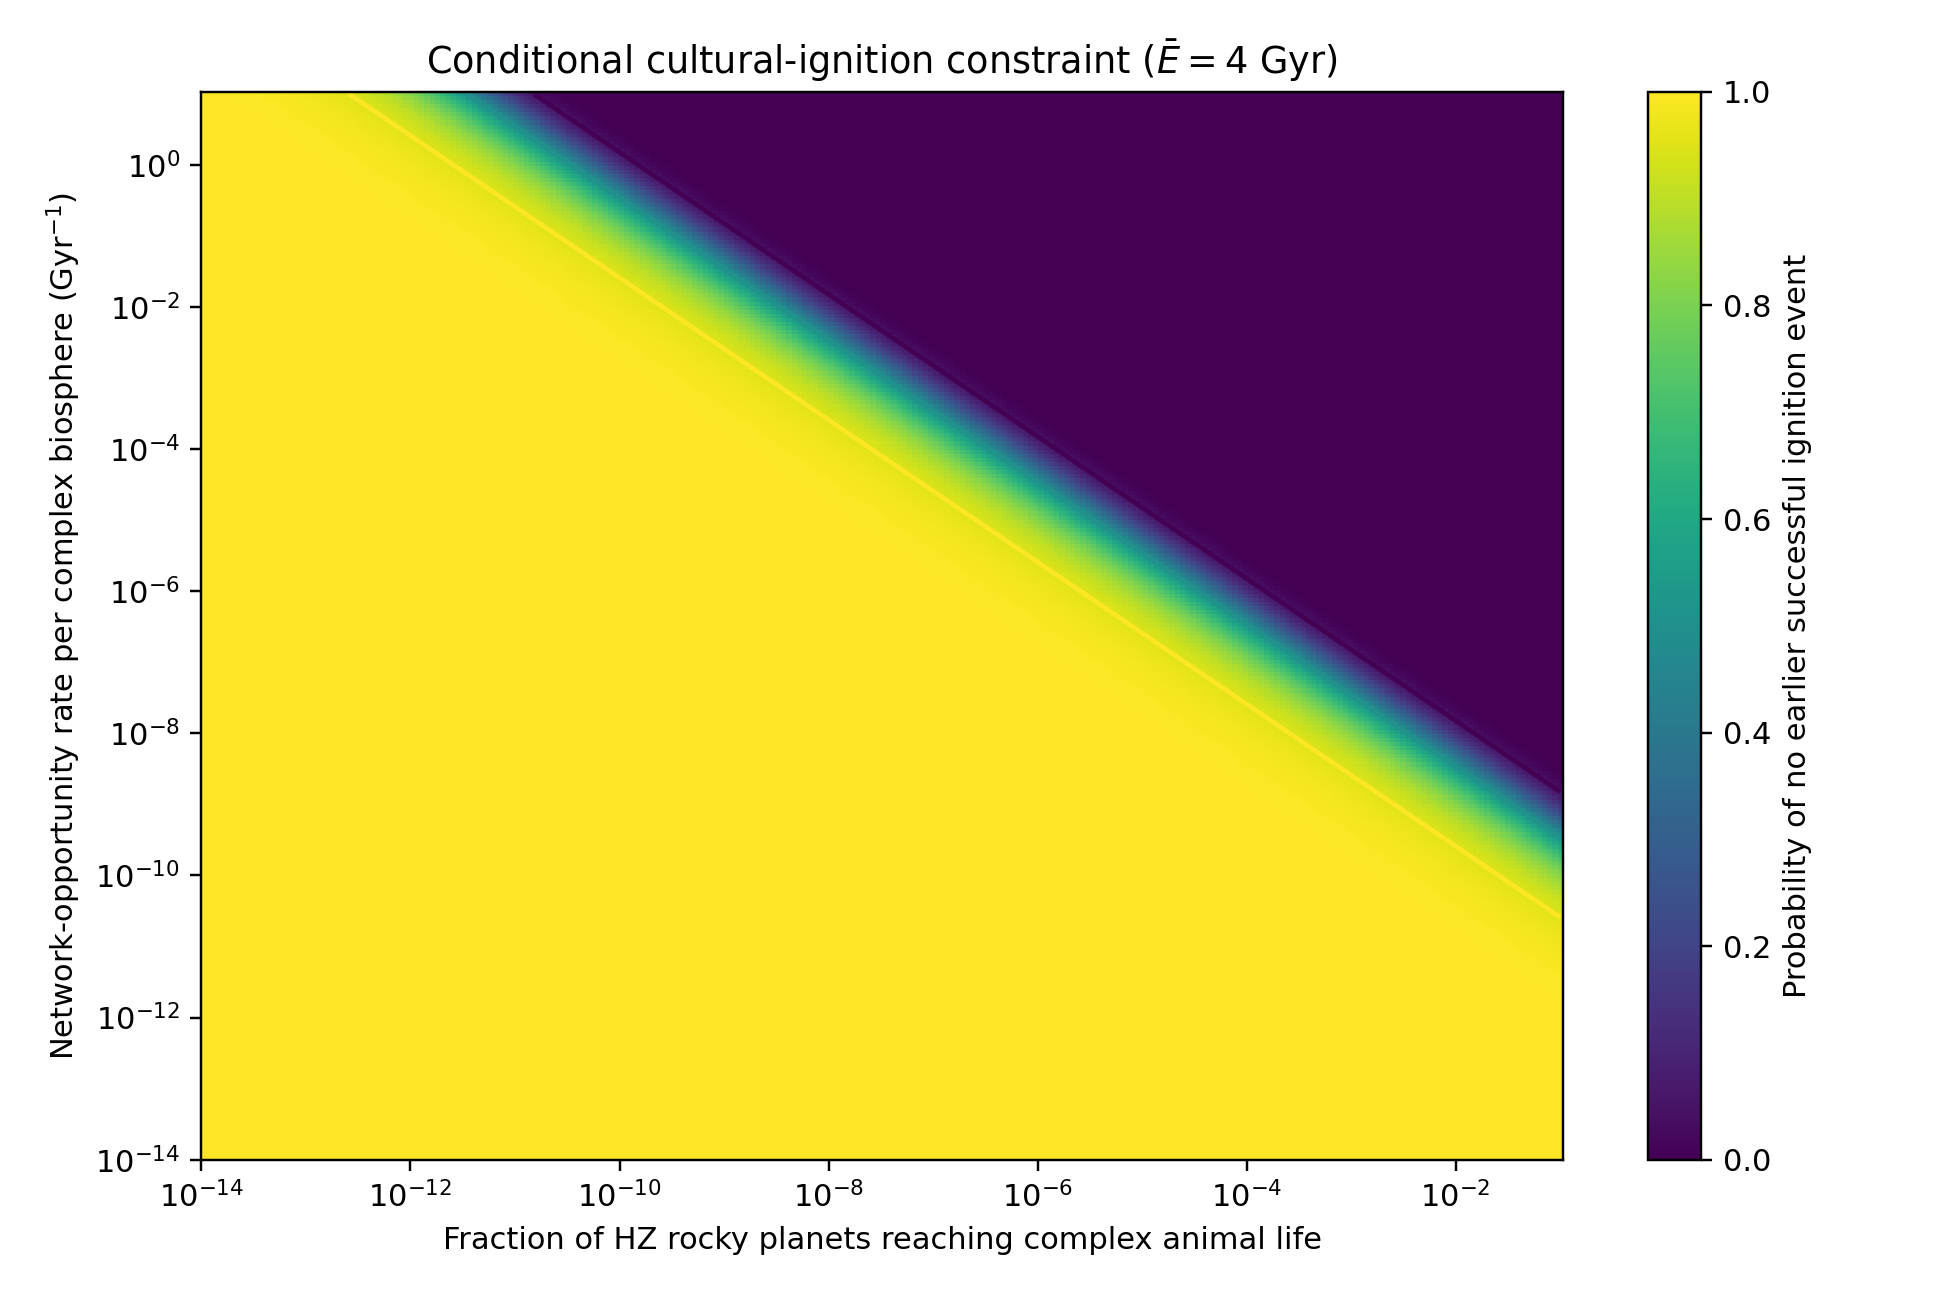
\includegraphics[width=0.94\textwidth]{figures/fig6.png}
\caption{Conditional probability of no earlier successful ignition event as a function of complex-biosphere prevalence and ignition-opportunity rate for the fiducial Galactic scenario.}
\label{fig:6}
\end{figure*}

These numbers are conditional scenario bounds, not estimates of extraterrestrial abundance. They demonstrate the degeneracy that any cultural Great Filter must confront: if complex biospheres are common and ignition opportunities recur frequently, even a network transition with \(P_{\rm ignite}\) near one-half would predict many predecessors. Conversely, a rare conjunction of complex life, suitable network structure and sustained teaching can make a late local ignition compatible with cosmic silence.

\section{DISCUSSION}

\subsection{Intelligence need not imply a technological society}

For the reference parameters and simulated horizon, the model can remain below the technological threshold despite agents with innovation, social learning and local traditions. This separation between individual cognition and collective accumulation is consistent with collective-brain and cultural-brain accounts \citep{muthukrishna2018} and with models of open-ended cultural evolution \citep{winters2026}. The limiting step is simultaneous preservation and recombination of complementary, prerequisite-rich skills. This supports a network-level interpretation of technological intelligence: the relevant unit is a metapopulation and its information architecture rather than an isolated brain.

Metastable accumulation and loss of innovations are also expected in punctuated cultural models \citep{kolodny2015}. The mechanism complements, rather than duplicates, the algorithmic-bottleneck proposal of \citet{prokopenko2026}. Their symbolic-language threshold concerns a structural coding transition. Here teaching, communication and model sampling are mechanistically represented as continuous population processes, and the transition probability is propagated into a cosmic population constraint. Symbolic communication may be one physical route by which real populations increase fidelity and access to external cultural models.

\subsection{Archaeology supplies compatibility, not a unique causal calibration}

The robust Middle Pleistocene change point is consistent with the original archaeological conclusion of \citet{paige2024}, but the current model does not identify contact as its cause. Procedural-unit sequences are selected published descriptions, dates are uncertain and multiple records may share research traditions. Cluster bootstrap and leave-one-cluster-out analyses reduce but do not remove these limitations. A direct empirical test should jointly model procedural complexity, raw-material transport proportions, settlement density and temporal uncertainty using ROAD or regionally curated assemblages.

\subsection{Astrobiological interpretation}

Cosmic planet formation may have produced many candidate worlds before Earth, while the cosmic future may contain still more \citep{behroozi2015,loeb2016}. This weakens explanations that rely only on the late appearance of rocky planets. A cultural ignition filter instead acts after intelligence and can remain rare on old biospheres. It therefore offers a resolution class in which the Galaxy may contain complex or intelligent organisms without a correspondingly large population of technosignature-producing societies.

The absence of detected technosignatures is not itself a strong direct estimate of \(\Lambda_{\rm prior}\) because the searched fraction of the multidimensional SETI haystack remains limited \citep{wright2018}, and settlement models permit unvisited systems in some inhabited steady states \citep{carroll2019}. The probability-of-no-prior-event equation is consequently a conditional prior-population constraint, not a likelihood analysis of SETI observations.

\subsection{Limitations and falsifiable predictions}

The cultural domains, teaching functions, demographic structures and benefit coefficients are stylised. Population-size effects can be non-monotonic in experiment and model \citep{fay2019,walker2026}, so the exploratory scaling results should not be read as a universal monotone law. The global sensitivity analysis shows that learning fidelity, cognition-dependent copying and teaching strength dominate outcomes, but parameter values are not yet inferred from prehistoric populations. Network diversity is externally maintained by ecological specialisation. The cosmological exposure and planet counts are scenario choices, and \(f_{\rm complex}\) and \(r_{\rm opp}\) are unresolved.

The model predicts that stable increases in technological complexity should be preceded by increased access to non-local cultural models, especially long-range bridges that recombine complementary specialities; that early high-complexity episodes can be metastable and lost; and that teaching/fidelity proxies should rise before or together with sustained repertoire expansion. Archaeological tests can use raw-material sourcing, stylistic convergence, settlement connectivity and persistence of prerequisite-rich production sequences. Astrobiologically, the hypothesis predicts that individual intelligence and even tool traditions may be much more common than detectable technological societies.

\section{CONCLUSION}

A continuous-feedback agent model produces a robust, stochastic transition from distributed local traditions to persistent cumulative culture. The transition is robust to outcome definitions, is not confined to the reference population architecture, shifts across network architectures, and is not observed within the tested ablation grid when recombination, teaching or infrastructure feedback is removed. A Middle Pleistocene archaeological regime change is robustly present in an open procedural dataset but does not uniquely validate the network cause. Embedding the local transition in a Poisson Galactic population model turns the mechanism into a quantitative candidate Great Filter: it constrains the joint prevalence of complex biospheres and cultural-ignition opportunities without claiming that humanity is demonstrably first. The resulting research programme links archaeological inference, cultural-evolution theory, astrobiology and the cosmological timing of technological societies.


\section*{DATA AND CODE AVAILABILITY}
The code, preprocessing script, frozen input tables, ensemble outputs, analysis scripts, software-environment files and figures required to reproduce the reported analyses are provided in the accompanying versioned research archive. A permanent repository URL or DOI will replace this sentence after public deposit; the submitted archive is also available from the corresponding author.

\section*{FUNDING}
This research received no specific grant from any funding agency in the public, commercial or not-for-profit sectors.

\section*{CONFLICT OF INTEREST}
The author declares no competing interests.

\acknowledgements{The author thanks the creators of the open archaeological datasets and open-source scientific software used in this study. OpenAI ChatGPT was used interactively during exploratory model formulation, code drafting, statistical-workflow design and language editing. The author executed and inspected the analyses, revised the code and manuscript, verified the cited sources and numerical results, and assumes full responsibility for the work.}

\newcommand\eprint{in press }
\bibsep=0pt
{\small\bibliographystyle{aa_url_saj}\bibliography{references}}
\clearpage
\end{document}
